 \documentclass[12pt,relax]{EpetraUserGuide}
\usepackage{array}
    \title{\EpetraTM{} User Guide}
\SANDsubtitle{}

    \author{Michael A. Heroux \\
      	  Computational Mathematics \& Algorithms Department \\
	    Robert J. Hoekstra\\
      	  rjh:GroupName \\
         Alan Williams \\
            aw:GroupName \\
	    Sandia National Laboratories\\
	    P.O. Box 5800\\
	    Albuquerque, NM 87185-1110 \\
	    maherou@sandia.gov \\
	    rjhoeks@sandia.gov \\
	    william@sandia.gov \\
	 }

    % There is a "Printed" date on the title page of a SAND report, so
    % the generic \date should generally be empty.
    \date{\today} % Remove ``\today'' in final version


\SANDnum{SAND2003-xxxx}
\SANDprintDate{April 2003}
\SANDauthor{Michael A. Heroux, Robert J. Hoekstra, Alan Williams, Sandia National Laboratories}


\SANDreleaseType{Unlimited Release}


\SANDdistcategory{UC-999}    

\begin{document}
\maketitle

\begin{abstract}

The \TrilinosTM{} Project is an effort to facilitate the design, development,
integration and ongoing support of mathematical software libraries.
One special Trilinos package is \EpetraTM{}.  Epetra provides a collections of
vector, graph and matrix objects that can be used on serial
and parallel computers.  It is designed to make construction, use and redistribution
of these objects as efficient and easy as possible.  Epetra objects are compatible with all
other Trilinos packages, including all linear, nonlinear and eigen solvers and all
preconditioners packages.  It also implements all Trilinos abstract interfaces and 
provides access to the Zoltan~\cite{zoltan-ug} load balancing package, and an object-oriented
interface to the BLAS~\cite{BLAS1,BLAS2,BLAS3} and LAPACK~\cite{lapack}.


This user guide is designed to address two types of users: 
(i) those who
are primarily interested in using already-constructed Epetra objects (such as 
numerical algorithm developers who want to implement algorithms via 
operations on Epetra vector, graph and matrix objects) and 
(ii) those who, in addition to using Epetra
objects, are also constructing Epetra vector, graphs and matrices.  This group
includes application developers who are constructing these objects for the purpose
of solving linear, nonlinear and eigensystems.

\end{abstract}


\section*{Acknowledgement}
The authors would like to acknowledge the support of the ASCI and LDRD 
programs that funded development of Trilinos and recognize all Trilinos 
contributors: Teri Barth, Roscoe A. Bartlett, David Day, Bob Heaphy, 
Robert Hoekstra, Jonathan Hu, Tammy Kolda, Richard Lehoucq, Kevin Long, 
Roger Pawlowski, Andrew Rothfuss, Andrew Salinger, Ken Stanley, Ray 
Tuminaro and Jim Willenbring.

\clearpage
\tableofcontents
\listoffigures
\listoftables

\clearpage

\section*{Nomenclature}
\addcontentsline{toc}{section}{Nomenclature}
\begin{itemize}
\item[Trilinos]
The name of the project of which Epetra is one of the packages.  Also a Greek term which,
loosely translated means ``a string of pearls,'' 
meant to evoke an image that each Trilinos package is a pearl in its 
own right, but is even more valuable when combined with other 
packages.
\item[Petra]
A Greek term meaning ``foundation.''  Trilinos has three Petra 
libraries: Epetra, Tpetra and Jpetra that provide basic classes 
for constructing and manipulating matrix, graph and vector
objects.  Epetra is the current production version that is
split into two packages, one core and one extensions.
\item[Comm Object]
An instance of one of the Epetra Comm classes.  Presently we support
an MPI, Serial and SMP/MPI implementation of the base Epetra_Comm interface.
\item[Map Object] 
Object-oriented algebraic preconditioner, compatible with 
Epetra and AztecOO.
\end{itemize}

NOTE: Add section on repeated use of Epetra objects.


\section{Introduction}
\label{Section:Introduction}
The Trilinos Project is an effort to facilitate the design, development,
integration and ongoing support of mathematical software libraries.
Trilinos provides a framework and set of tools for document and source code control,
software issue tracking, developer and user communication, automatic
testing, portable configuration and building, and software
distribution.  Trilinos also provides a set of core utility libraries
that provide common vector, graph and matrix capabilities, as well as
a common abstract interface for applications to access any appropriate
Trilinos package.

A new software capability is introduced into Trilinos as a {\it
package}.  A Trilinos package is an integral unit usually developed by
a small team of experts in a particular algorithms area such as
algebraic preconditioners, nonlinear solvers, etc.

The overall objective of Trilinos is to promote rapid development and
deployment of high-quality, state-of-the-art mathematical software in
an environment that supports interoperability of packages while
preserving package independence.  The Trilinos design allows 
individual packages to grow and mature autonomously to the extent the 
algorithms and package developers dictate. 

The Trilinos Developers Guide is meant to assist new and existing
Trilinos package developers.  Topics covered include how to configure and 
build Trilinos, what is required to integrate an existing package into Trilinos
and examples of how those requirements can be met, as well as what
tools and services are 
available to Trilinos packages.  Also discussed are some common practices that 
are followed by many Trilinos package developers.  Finally, a snapshot
of current Trilinos packages and their iteroperability status
is provided, along with a list of supported computer platforms.

For a higher-level view of the Trilinos project, please see An Overview
of the Trilinos Project~\cite{TrilinosOverview}. The current set of
packages in Trilinos is shown in Figure~\ref{Figure:TrilinosPackages}.
\begin{figure}
%\begin{center}
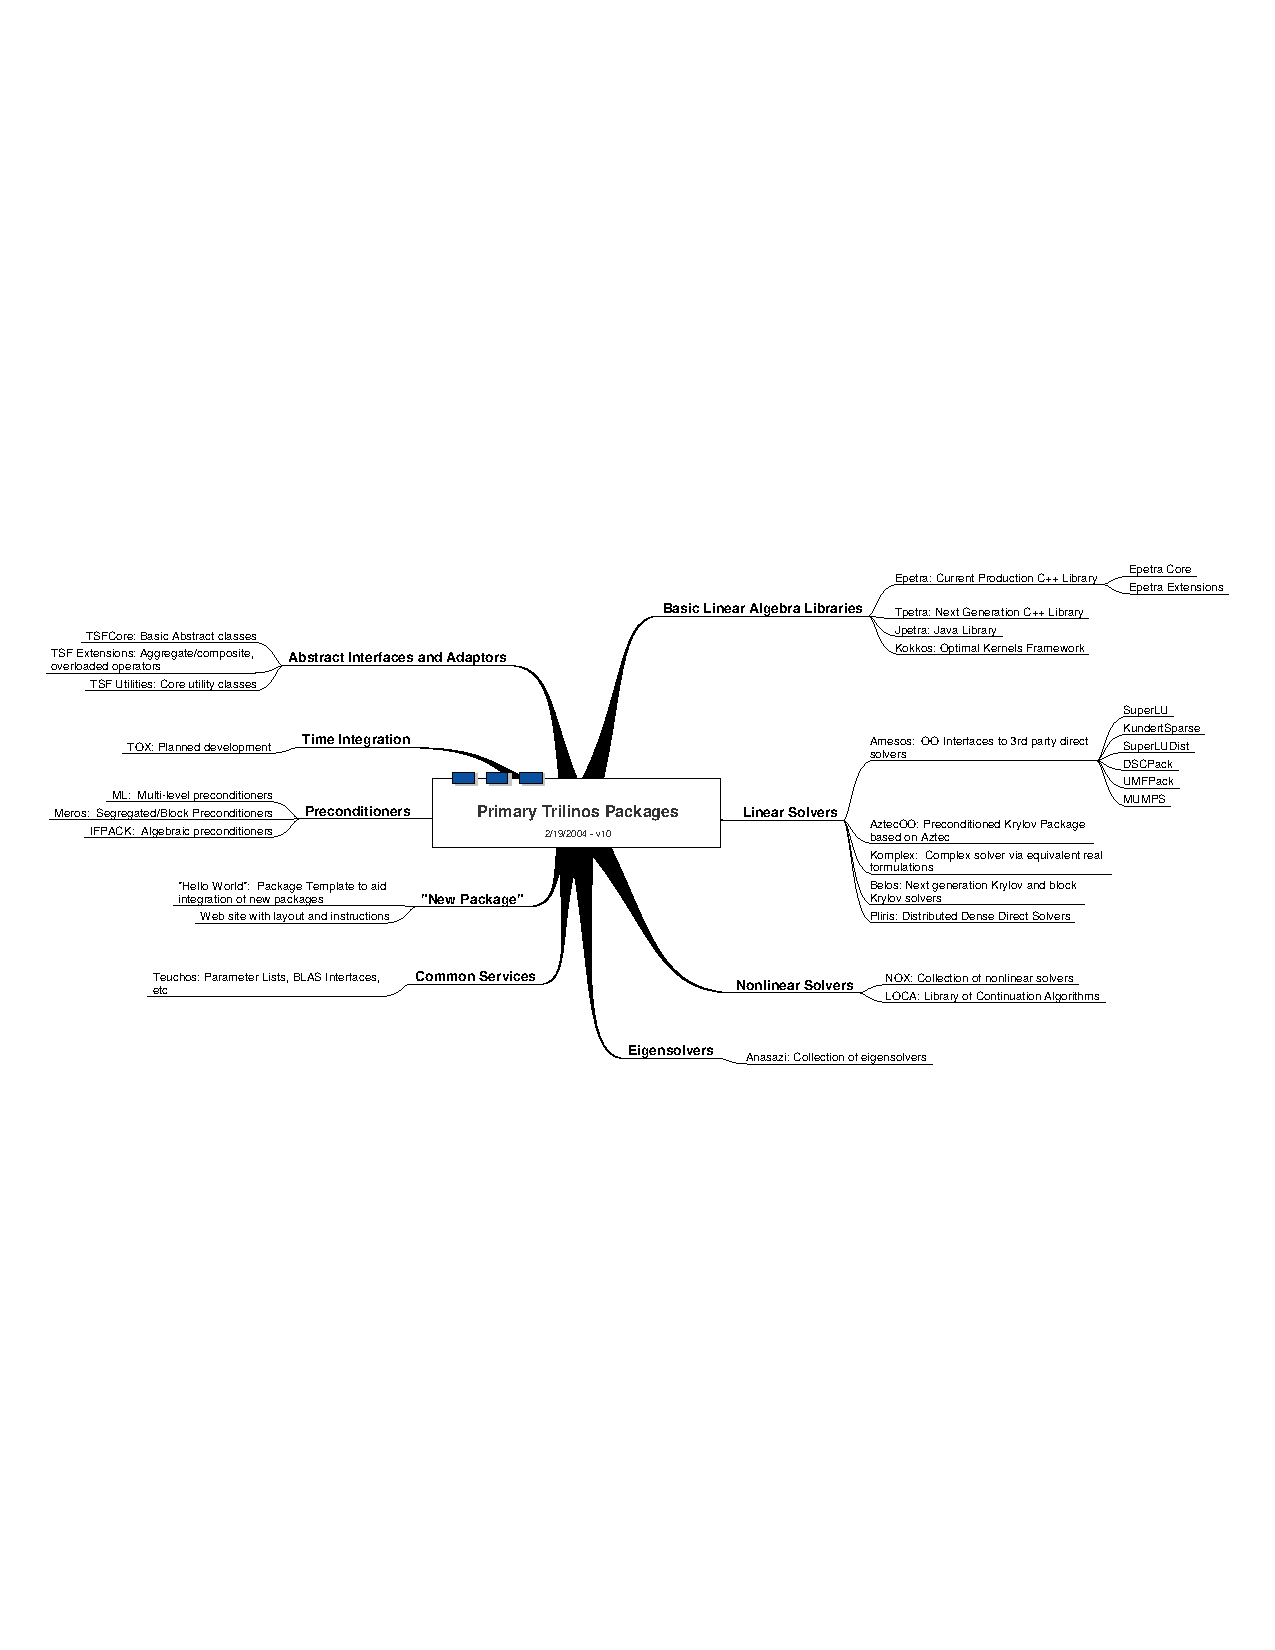
\includegraphics[height=6in,angle=270]{TrilinosPackagesDiagram}
%\end{center}
\label{Figure:TrilinosPackages}
\caption{Current collection of Trilinos Packages}
\end{figure}

\subsection{How To Use This Guide}

Although all sections of this guide will be useful to most developers,
it is worth mentioning that 
this guide supports three types of development activities:
\begin{enumerate}
\item New Project: Development of a new package using little or no
existing software as a base.  All sections of this guide are
appropriate reading.
\item Integration of an existing third-party software: In this case,
existing software is being imported into the Trilinos framework.  In
this case, Section~\ref{Section:IntegratingPackages} is particularly
important, as are Sections~\ref{Section:PackageRequirements},
~\ref{Section:AvailableServices} and~\ref{Section:EpetraAndTSF}.
\item Ongoing development:  For existing Trilinos package developers,
Sections~\ref{Section:PackageRequirements}
and~\ref{Section:AvailableServices} are designed as a reference for
software engineering practices and policies for Trilinos development.
\end{enumerate}

\subsection{Typographical Conventions}

Our typographical conventions are found in
Table~\ref{Table:TypoConventions}.
\begin{table}[ht]
\scriptsize
\begin{center}
\begin{tabular}{|l|l|p{2.0in}|} \hline
Notation & Example & Description \\ \hline
\InlineCommand{Verbatim text} & \InlineCommand{../configure --enable-mpi} & 
Commands, directory and file name examples, and other text associated
with text displayed in a computer terminal window. \\ \hline
\InlineCommand{CAPITALIZED\_TEXT} & \InlineCommand{CXX\_FLAGS} & 
Environment variables used to configure how tools such as compilers behave. \\ \hline
\InlineCommand{[text in angle brackets]} & \InlineCommand{../configure
<user parameters>} & 
Optional parameters. \\ \hline
\end{tabular}
\end{center}
\caption{\label{Table:TypoConventions} Typographical Conventions for This Document.}

\end{table}


\section{Getting Started}
\label{Section:GettingStarted}
This chapter covers some of the basics that a developer will need to know when 
beginning to work on the Trilinos project.  We address how to configure and 
build Trilinos, as well as how to add files to an existing package.

\subsection{Recommended Build Directory Structure}

Via Autoconf and Automake the Trilinos configuration facilities
provide a great deal of flexibility for configuring and building the
existing Trilinos packages.  However, unless you have prior experience
with Autotools, we recommend the following process to build and
maintain your local builds of Trilinos

To start, we defined two useful terms:
\begin{itemize}
\item Source tree - The directory structure where source files are found.  A source 
tree is obtained by expanding a distribution tar ball, or by checking 
out a copy of the Trilinos repository.  
\item Build tree - The directory structure where object and library files, as well 
as executables are located.  
\end{itemize}
 
Although it is possible to run \InlineCommand{configure} from the source tree (in 
the directory where the configure file is located), we recommend that a 
user have separate build trees.  The greatest advantage to having a separate 
build tree is that multiple builds of the libraries can be maintained
from the same source tree, for 
example, serial and parallel libraries.  A less obvious advantage is that 
there can be problems with configuring in a 'dirty' directory (one that has 
already been configured in).

	Setting up a build tree is straight-forward.
Figure~\ref{Figure:TrilinosDirectoryStructure} illustrates the
\begin{figure}
\begin{center}
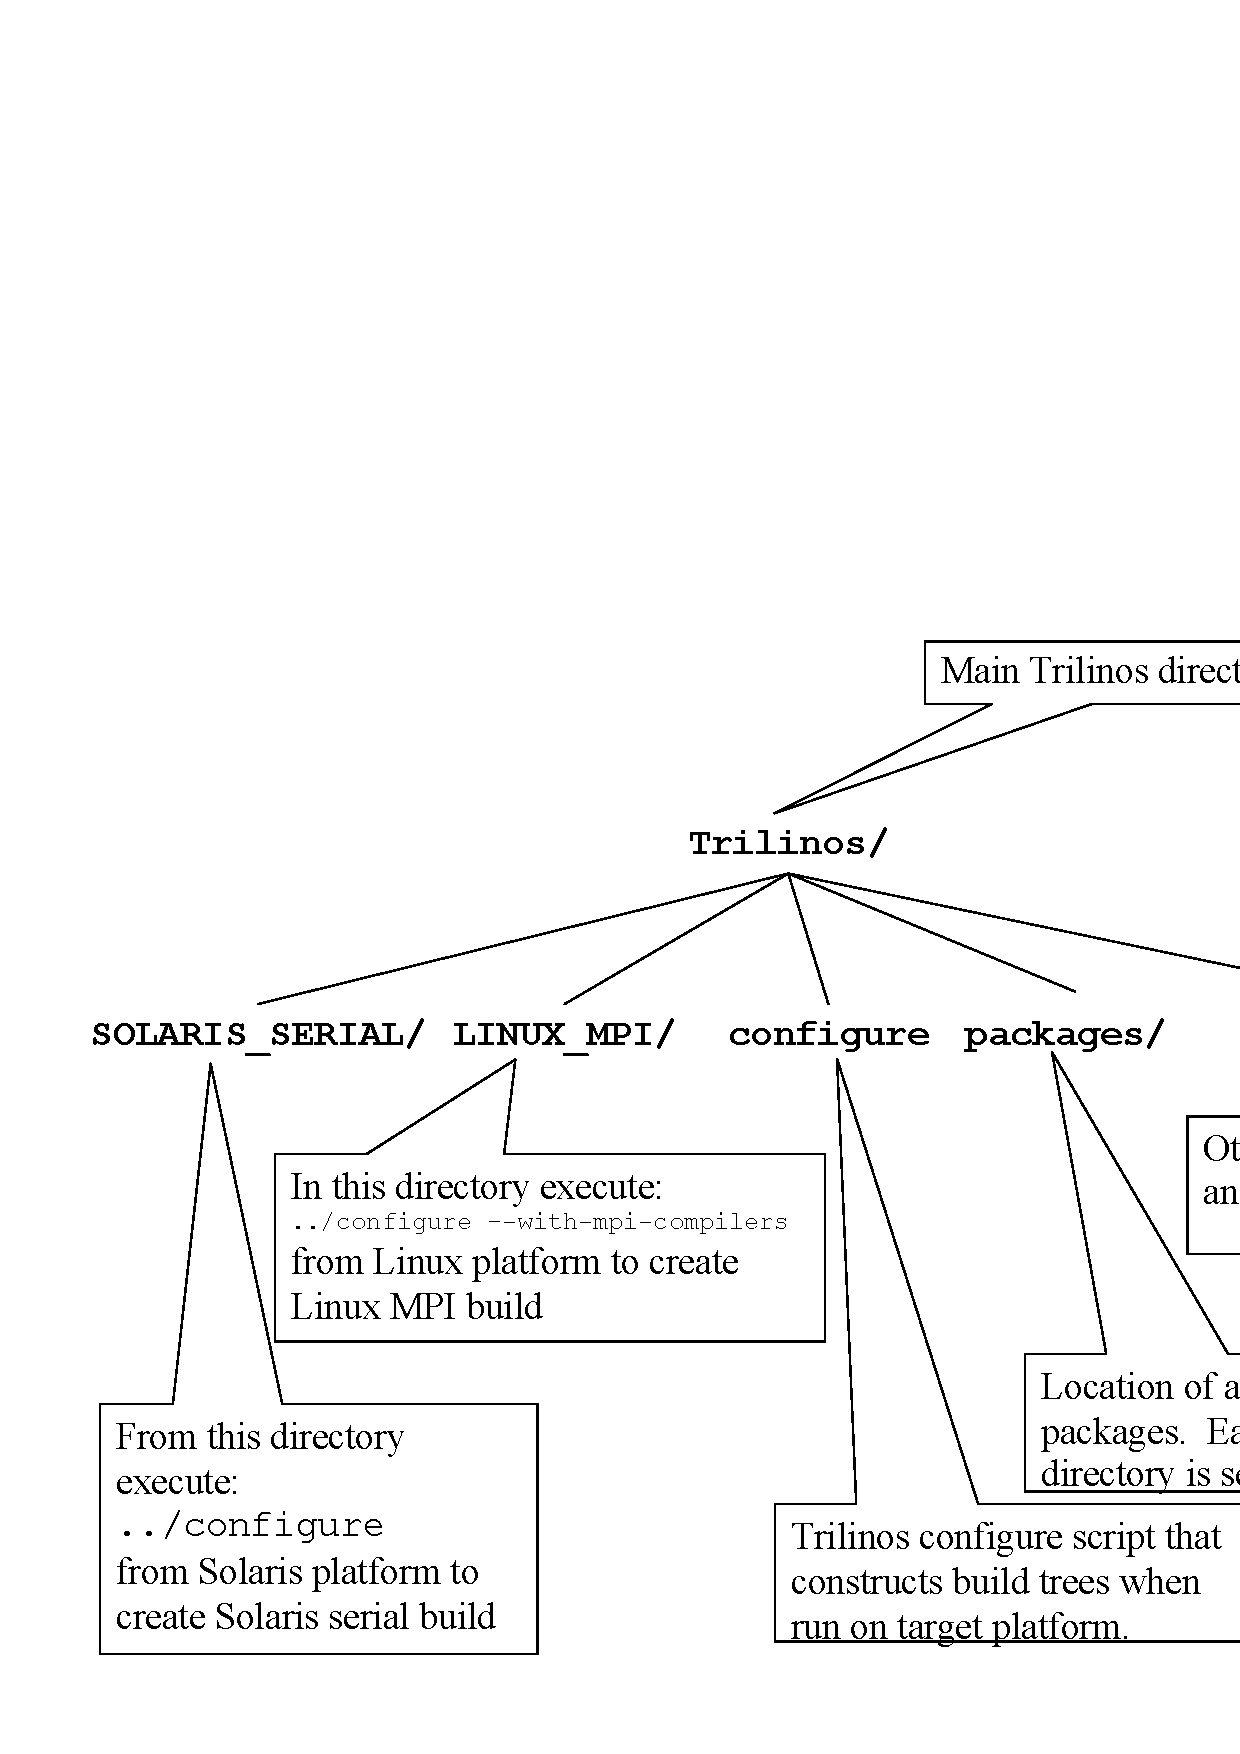
\includegraphics[width=4in,angle=270]{TrilinosDirectoryStructure}
\end{center}
\label{Figure:TrilinosDirectoryStructure}
\caption{Recommended Layout for Trilinos Build Directories}
\end{figure}recommended layout.  First, \InlineCommand{cd} to the highest 
directory in the source tree (Trilinos for a repository copy, Trilinos-3.0.1 
for a distribution).  Now, make a new directory - for an MPI build
on a Linux platform, a 
typical name could be \InlineDirectory{LINUX\_MPI}.  
Finally \InlineDirectory{cd} into that dirctory.  In summary:

\begin{verbatim}
       cd Trilinos
       mkdir LINUX_MPI
       cd LINUX_MPI
       ../configure --enable-mpi
       make
\end{verbatim}
At this point, the MPI version of Trilinos on a Linux platform is
built and completely contained in the \InlineDirectory{LINUX\_MPI}
directory.  No files outside this directory have been modified.  This
procedure can be repeated for any number of build targets.

{\bf Note:} Although we recommend the above location for build trees,
they can be set up anywhere.

\subsection{Configuring Trilinos}
\label{Subsection:ConfiguringTrilinos}
	To configure from a remote build tree, simply run the configure script 
in source tree from the root of the build tree.  In the example above, cd to 
the SERIAL directory and type 
\DisplayCommand{../configure <options as described below>}

A detailed list of configure options can be seen by typing
\DisplayCommand{configure --help=recursive} from the top level of the 
source tree.  This will display the help page for the Trilinos level as well as all 
Trilinos packages that use autoconf and automake.  The output from this command
is quite extensive.  To view the help page for an individual package, cd to 
the home directory for the package in the source tree and type 
\DisplayCommand{configure --help} 
This command will also display the help page for Trilinos level 
options when used from the Trilinos home directory in the source tree.


	The user needs to provide two important pieces of information at this 
stage.  First, the user needs to describe what kind of a build is needed.  For 
instance, serial or mpi, all of the packages, or just a proper subset.  

	For example, to configure for serial libraries, no action is necessary,
but to configure for parallel libraries, a user must append appropriate 
arguments to the configure invocation line as described in the "Configure 
Options" section.

	Also, to build the default set of Trilinos libraries, no action is 
necessary, but to exclude a default package, komplex for example, a user must 
append \InlineCommand{--disable-komplex} to the configure invocation  line.  
Similarly, to include a package that is not currently built by default, NOX 
for example, users must append \InlineCommand{--enable-nox} to the configure 
invocation line.  It is recommended that users always configure from the 
Trilinos level and use \InlineCommand{--disable-<package>} as necessary, 
rather than trying to configure from a lower level.  To see which packages 
build by default and which ones don't, simply cd to the Trilinos home 
directory and type \DisplayCommand{configure --help}.

NOTE: Ifpack is divided into old and new portions.  Future ifpack developments 
will replace all of old ifpack, but at this time some users will need to append
\InlineCommand{--enable-oldifpack} to the configure line.

NOTE: The configure process is set up to detect when a 
\InlineCommand{--disable-<package>} option would break a package dependency.  
For example, ifpack depends on epetra, so if a user wants to build ifpack, but 
types \InlineCommand{--disable-epetra}, epetra will be configured and built 
anyway.  However, some of the tests and examples have different dependencies 
than the core package.  It is possible that not all of these dependencies have 
been accounted for.  Please submit a bug report for any problems found with 
this matter.

	To install libraries and header files in a particular location, 
use \InlineCommand{--prefix=<dir>} on the configure line.  If this option is 
used, libraries will be located in \InlineDirectory{<dir>/lib} and header files in 
\InlineDirectory{<dir>/include/<package>}.

	The second important piece of information that a user must provide at 
this stage is the name and or location of anything that autotools needs and 
cannot find on its own.  Also, if autotools selects, for example, the wrong 
blas library by default, the user must indicate which blas library to use.  
Other more obscure issues dealing with enjoyable topics such as standard 
noncompliance are also dealt with here.  If all required libraries (often 
blas, and lapack) are located in standard places, try configuring with what 
you have.

	For a machine that requires additional configure line options, a good 
place to start is Trilinos(-3.0.1)/config.  There are configure invocation 
scripts here for various platforms.  These scripts are named using the 
following naming convention:
\InlineCommand{arch\_comm\_machine}.
For example \InlineCommand{sgi64\_mpi\_atlantis}.  Note that these scripts are examples 
only.  Users should not necessarily expect to be able to find the perfect 
script and use it, but rather should choose a script for a similar machine, 
examine the options used in the script and figure out if those options make 
sense for the case at hand.  Some of the scripts in the repository are not 
always up to date.  If a user submits a script for a machine that few Trilinos 
developers have an account on, that script may become obsolete if it is not 
updated by the user who submitted it.  For reasons such as this, these scripts 
tend to be primarily useful for the values of options such as \InlineCommand{LDFLAGS}, 
\InlineCommand{CPPFLAGS}, and \InlineCommand{CXXFLAGS}.  

Users who create scripts for other machines are encouraged to check them into 
the repository for the benefit of other users.  Users who do not have access to
the repository can send their scripts to \InlineCommand{jmwille@sandia.gov}.

\subsection{Building Trilinos}

If the configure stage completed successfully, just type \DisplayCommand{make}
 and if 
\InlineCommand{--prefix} was specified, \DisplayCommand{make install}

The following section describes the configuration options mentioned above that 
are common to all Trilinos packages.  These options DO NOT cover all options 
for all Trilinos packages.

\subsection{Trilinos Configuration Options}

The following options apply to all Trilinos packages unless 
the option doesn't make sense for a particular package (for example, a 
package that does not include any Fortran code will not be sensitive to 
\InlineCommand{F77=g77}), or otherwise noted.  For options specific to 
individual package, cd to the home directory of the source code of the 
individual package and type \DisplayCommand{configure --help}.

Basic Options

\begin{itemize}
\item \InlineCommand{--enable-debug} 

(Nox only.)  This turns on compiler debugger flags. It has 
not been fully tested. As an alternate, specify CXXFLAGS on the 
                 configure line.

\item \InlineCommand{--enable-opt}

(Nox only.)  This turns on compiler optimization flags. It 
has not been fully tested. As an alternate, specify CXXFLAGS on the 
                 configure line. 

\item \InlineCommand{--with-cppflags}

Specify additional preprocessor flags (e.g., "-Dflag -Idir") 

\item \InlineCommand{--with-cxxflags}

Specify additional C++ flags 

\item \InlineCommand{--with-ldflags}

Specify additional linker flags (e.g., "-Ldir") 

\item \InlineCommand{--with-ar}

Specify a special archiver command, the default is "ar cru". 
\end{itemize}

 Influential Environmental Variables

\begin{itemize}
\item \InlineCommand{CC}

C compiler command.

\item \InlineCommand{CFLAGS}

C compiler flags.

\item \InlineCommand{CXX}

C++ compiler command.

\item \InlineCommand{CXXFLAGS}

C++ compiler flags.

\item \InlineCommand{LDFLAGS}

Specify linker flags.

\item \InlineCommand{CPPFLAGS}

C/C++ preprocessor flags.

\item \InlineCommand{CXXCPP}

C++ preprocessor.

\item \InlineCommand{F77}

Fortran 77 compiler command.

\item \InlineCommand{FFLAGS}

Fortran 77 compiler flags.
\end{itemize}

MPI-Related Options

\begin{itemize}
\item \InlineCommand{--enable-mpi}

Enables MPI mode. Defines HAVE\_MPI in the (Package)\_Config.h file. Will test 
for the ability to preprocess the MPI header file and may test ability to link 
with MPI.  This option is rarely necessary as many of the below options also 
turn MPI on.  

\item \InlineCommand{--with-mpi-compilers}

Sets the MPI c++ compiler = mpicxx (or mpiCC if mpicxx not available), 
the MPI C compiler = mpicc and the MPI Fortran compiler = mpif77.  
Automatically enables MPI mode.  To use compilers other than these, 
specify mpi locations with the below options.  If none of these options 
are necessary, don't forget to use --enable-mpi.  CXX, CC, and F77 may also 
have to be set if autoconf does not choose the correct compilers by default.

\item \InlineCommand{--with-mpi=MPIROOT}

Specify the MPI root directory. Automatically enables MPI mode.  If this 
option is set, \InlineCommand{--with-mpi-incdir} and 
\InlineCommand{--with-mpi-libdir} should not be used.  
\InlineCommand{--with-mpi} is meant to be a shortcut for setting 
\InlineCommand{--with-mpi-libdir=MPIROOT/lib} 
and \InlineCommand{--with-mpi-incdir=MPIROOT/include}.  Use these two options instead if 
these default locations are not correct.

\item \InlineCommand{--with-mpi-libdir=DIR}

Specify the MPI libraries location. Defaults to MPIROOT/lib if --with-mpi 
is specified. If multiple directories must be specified, try 
\InlineCommand{--with-ldflags="-L<dir1> -L<dir2>"} instead. 

\item \InlineCommand{--with-mpi-libs="LIBS"} 

Specify the MPI libraries. Defaults to \InlineCommand{"-lmpi"}
 if either\InlineCommand{ --with-mpi} or 
\InlineCommand{--with-mpi-libdir} is specified.

\item \InlineCommand{--with-mpi-incdir=DIR}

Specify the MPI include files location. Defaults to \InlineDirectory{MPIROOT/include} if 
\InlineCommand{--with-mpi} is specified. If multiple directories  must be specified, try 
\InlineCommand{--with-cppflags="-I<dir1> -I<dir2>"} instead.
\end{itemize}

Developer-Related Options
\begin{itemize}
\item \InlineCommand{--enable-maintainer-mode}

Enable make rules and dependencies not useful (and sometimes confusing) to 
the casual installer.
\end{itemize}

Other important notes about the configure/build process.
\begin{itemize}
\item Any code that links to Trilinos should define \InlineCommand{HAVE\_CONFIG\_H}.
\item Often the output from configure will be inadequate for diagnosing 
problems.  A developer should look (in the buildtree) at the config.log file 
for the package that failed to configure properly.  To figure out which 
package failed to configure, simply look at the bottom of the output from the 
'configure' command.  One of the last lines should say something like:

\begin{verbatim}
    configure: error: /bin/sh '../../../packages/epetra/configure' 
    failed for packages/epetra.
\end{verbatim}

This particular error indicates to look in \InlineDirectory{packages/epetra/config.log}.  This 
file is useful for developers trying to build Trilinos, and those who are 
adding or editing autoconf-specific files such as configure.ac.
\end{itemize}

\subsection{Adding and Removing Source Files}

Commonly a developer needs to add files to or remove files from a Trilinos 
package.  We outline the steps for adding or removing source files from a 
Trilinos package that uses Autotools.  The below outline assumes the simple 
addition or removal of files.  Special situations such as adding header file 
or library dependencies to a Trilinos package or conditionally compiling new 
files require a more complicated process.
\begin{enumerate}
\item Obtain the supported versions of Autoconf and Automake.

The current supported versions of Autoconf and Automake are documented in 
the Trilinos repository.  Trilinos/config/AutotoolsVersionInfo contains the 
information.  The Trilinos team does not attempt to keep up with the latest 
versions of Autoconf and Automake, so please do not assume that the most 
recent versions are supported.  The supported versions of Autoconf and 
Automake can always be found on software.sandia.gov.  This makes software a 
good machine to bootstrap on.  However, software does not currently have an
mpi implementation installed.

\item Update source code from Trilinos repository

Obtain the most current version of Trilinos (for the branch being worked on).  
First, cd to the top Trilinos directory, then type

\DisplayCommand{cvs -q update -dP}

\item Add new files to or remove obsolete files from the Trilinos repository

To add new files abc.cpp and abc.h to the Trilinos repository, cd to the 
directory in which the files are located in a checked out version of the 
Trilinos repository and type

\DisplayCommand{cvs add abc.cpp abc.h}

To remove the same files, type

\DisplayCommand{cvs remove abc.cpp abc.h}

The above commands do not actually add the files to or remove the files 
from the repository, but simply prepare for the addition or removal of the 
files.  The files will really be added or removed later using 
\InlineCommand{cvs commit}.  However, this is a necessary step in the process.

\item List new files in or remove obsolete files from Makefile.am

New source files should be placed into a category in the appropriate 
Makefile.am.  Typically, the directory in which the new files are located will 
contain a Makefile.am.  If not, the appropriate Makefile.am will be found in 
the Makefile.am that is in the parent directory directly above the directory 
in which the new files are located.  The number of possibly categories to add 
files to varies a lot.  For a test or example a developer will typically just 
add the files directly to a SOURCES primary.  For a Trilinos package, there 
may be several categores of files.  For example UTIL, CORE, and DIST, to name 
a few.  Do not worry too much about which macro category to add the files to.  
The categories are simply a way to sort files into logical groups.  To remove 
files from the build process, simply delete the file names from the 
appropriate Makefile.am.

\item Bootstrap

First, cd to the top-level directory of the appropriate Trilinos package.  
For example Trilinos/packages/epetra.  Then type 

\DisplayCommand{./bootstrap}

The process should complete without any errors, but the following warnings do 
commonly occur:

\begin{verbatim}
configure.ac:9: warning: do not use m4_patsubst: use patsubst or m4_bpatsubst
configure.ac:184: warning: do not use m4_regexp: use regexp or m4_bregexp
\end{verbatim}

\item Test the new code

Reconfigure and rebuild the Trilinos package.  Perform tests associated with 
the new code, as well as the rest of the tests for the package to insure that 
both the new code works and existing code has not been broken.  When changes 
could possibly affect other packages, tests for affected packages should also 
be run.

\item Update source code from Trilinos repository

Didn't we just do this?  Yes, but there are two good reasons to do it again.

Other developers could have committed changes during the past several 
steps of this process.  Though is not likely, it is worth checking.  If 
changes were committed, minimally the testing step will need to be redone.  
If files related to configuring or building were modified, more will have to 
be done if collisions occur.  Some of the possibilities are beyond the scope 
of this introductory document, however we will briefly discuss the most 
common collision scenario.  Typically the generated files will contain 
collisions (for example configure, Makefile.in, or aclocal.m4), while the 
changes in the files created by developers (for example configure.ac or 
Makefile.am) will be successfully merged by CVS.  In this case, the best 
course of action is to remove the files with collisions, cd to the top level 
of the Trilinos package, perform a cvs update, and then begin the above 
process again from ``Bootstrap'' step.  As long as the changes are merged in 
the non-generated files, bootstrapping should resolve the problem.

An even better reason to update again before committing changes is to avoid 
confusion.  After a bootstrap, all of the generated files will get an updated 
timestamp, but in most cases only some of the files will actually be 
modified.  If a developer commits changes before updating, all of the 
generated files will be viewed as having been modified.  This is bad for 
several reasons.  One of the most important is that when committing changes, a 
developer should always verify that the list of files that are about to be 
committed makes sense.  The list is guaranteed to not make sense if files are 
going to be committed that have not been changed.  A cvs update will check to 
see if the file has really been changed or if it simply has a new timestamp.

\item Commit the changes to the Trilinos repository

Once all of the above steps are completed, the final step is to commit the 
changes to the repository.  Start by typing

\DisplayCommand{cvs commit}

Now, look at the list of files that are to be added, removed  or modified.  
It is easy to inadvertantly commit files.  It is also easy to forget to use 
\InlineCommand{cvs add}.  If a file has not been added, it will not show up on 
the list of files to be added.  Conversely, to remove a file, don't forget to 
use \InlineCommand{cvs remove}.  

Here are a few helpful tips to use when verifying the list of files 
to be committed.  First, make sure that all files you modified directly appear 
in the list.  Second, when modifying a Makefile.am, the corresponding 
Makefile.in will change also.  Third, when modifying configure.ac, configure 
will also change, but some Makefile.in files may also change when using macros 
such as AC\_SUBST.  Finally, when unsure about whether or not a 
file should be in the commit list, abort the commit by closing the edior 
without saving, and chosing \InlineCommand{abort}.  Then, if abc.cpp is in 
question, type 

\DisplayCommand{cvs diff abc.cpp}

Then look at the diff output and see if it makes sense for the changes that 
were made.  After verifying that all of the files that are in the list belong 
there, and that all files that belong in the list are, in fact, listed, remove 
unnecessary instances of ``CVS: `` from the log message and enter an 
appropriate description of the changes that are to be committed.  Don't forget 
to reference any appropriate Bugzilla bug numbers.  Further, detailed log 
messages make it easier to track problems in the future.  It is a good habit 
to indicate which tests were run before making the change.

Finally, save the file, and exit the CVS editor to commit the changes.

When using the above process to commit new source code, the new source must 
be functioning properly, otherwise the repository will not be stable.  
At the same time, developers are encouraged put new code into the repository 
during initial development.  This will ensure that work is backed up and 
provide version control.  When adding unstable code to the repository, only
two steps are necessary.  First, use the \InlineCommand{cvs add} command as 
mentioned above, and then modify the commit command slightly to commit only 
the new source by typing

\DisplayCommand{cvs commit newfile1.cpp newfile2.cpp}

Provided that the new files are not added to the make structure, the addition 
of the new files should not negatively affect the repository.  Distribution 
tarballs will even skip over the new source.  A common log message for this 
type of commit is simply ``Checking in for safe keeping; code is not yet 
funcitoning''.  Sometimes developers will include a short description of what 
the code will do when complete.
\end{enumerate}

\section{Services Available to Trilinos Packages}
\label{Section:AvailableServices}
A number of services exist for Trilinos packages.  Many of these 
services relate directly to some of the requirements and suggested practices 
for Trilinos packages.  For example the CVS repository is discussed below, and 
Trilinos packages must make use of this repository.  Also, Bonsai, Bugzilla 
and Mailman are all tools that relate to suggested practices.  (It should be 
noted that these services are not simply meant to satisfy SQE requirements.  
Rather, Bonsai, Bugzilla and Mailman have proved to be very useful tools.  
Using these tools together, along with the CVS repository, has led to a more 
time and cost effective code development process.)  For more information about 
any of the below services, please contact the Trilinos Project Leader.

\subsection{Configuration Management}
Autoconf~\cite{Autoconf},  Automake~\cite{Automake} and Libtool~\cite{Libtool} 
provide a robust, full-featured set of tools for building software across a 
broad set of platforms (see also the ``Goat Book''~\cite{GoatBook}).  Although 
these tools are not official standards, they are commonly used in many 
packages.  Many existing Trilinos packages use Autoconf and Automake (and will 
use Libtool in the future).  However, use of these tools is not required.

Package developers who are not currently using autotools, but would like
to, can get a jump start by using a Trilinos package called 
``new\_package''.  This trivial package exists for one primary purpose.  
It walks a developer through the process of setting up a package to 
configure and build using autotools.  General instructions for how to get 
started can be found in Trilinos/packages/new\_package/README.  Please note 
that new\_package is a work in progess, suggestions and contributions are 
welcome, especially for FAQ's.

Trilinos provides a set of M4~\cite{M4} macros that can be used by any other
package that wants to use Autoconf and Automake for configuring and
building libraries.  These macros perform common configuration tasks such as
locating a valid LAPACK~\cite{lapack} library, or checking for a user-
defined MPI C compiler.  The macros can be found in the Trilinos CVS 
repository in Trilinos/config.  These macros minimize the amount of redudant
 effort in using Autotools, and make it easier to apply a general change to 
the configure process for all packages.
\subsection{Regression Testing}
Trilinos provides a variety of regression
testing capabilities.  Within a number of Trilinos packages, we employ
``white box'' testing where detailed information about the software is
used and probed.  In addition, Trilinos performs ``black box'' testing
of packages via the Trilinos Solver Framework (TSF) virtual class
interfaces.  Any package that implements the TSF interfaces (see
Section~\ref{subsect:InteropTSF} below 
%**(Add this section)), 
can be tested via this black box
test environment.  ({\bf NOTE: Black box testing via TSF is not in
place at this time}
	\subsection{Periodic Testing}
Trilinos Packages that configure and build using Autotools can easily 
utilize the the Trilinos test harness.  The test harness performs a CVS update
(gets the most recent source code) every night and then builds the libraries
and runs any tests that have been integrated into the testharness.  
Currently the testharness only runs on Linux, IRIX64, and DEC/OSF1, but it 
will eventually run on 5-8 platforms.  Packages that have not ported to a 
particular platform can be excluded from the testing process on that 
platform.  Packages that do not have any tests integrated into the 
testharness can still benefit by ensuring that libraries build without 
errors.  Integrating existing tests into the testharness is not difficult.  
The process is discussed in Trilinos/testharness/HowToAddToTestHarness.  
Please note that this document is a work in progress.

\subsection{CVS Repository}
%**Add an appendix for a lot of this info.**
Trilinos source code is maintained in a CVS~\cite{CVS} repository.  It is 
very easy to add new packages to the repository.  Packages that already use 
CVS can even retain their CVS history!  To access the repository, one must 
have an account on software.sandia.gov.  Once an account has been granted, 
set the following two environment variables (replace ``your\_user\_name'' 
with your user name on software):

\DisplayCommand{CVSROOT :ext:your\_user\_name@software.sandia.gov:/space/CVS}
\DisplayCommand{CVS\_RSH ssh}

For those not familiar with CVS, below is a brief discussion covering some 
of the most common CVS commands.  For more information, see the Gnu CVS Home
Page~\cite{CVS}.

Checking Out a Working Copy

To get started, checkout a copy of the development branch of the repository.
(Releases branches can be obtained by by checking out the appropriate 
tagged version of the repository.)

\DisplayCommand{cvs checkout Trilinos}

Updating a Woring Copy
To update after a version has been obtained use the \InlineCommand{cvs update} 
command.  First, cd to the directory that is to be updated 
(usually the Trilinos root directory).  Then type:

\DisplayCommand{cvs -q update -dP}

The ``-q'' option means ``be somewhat quiet''.  Try the command without this
option to see what it does.  

The ``-d'' option means to get any new directories.  For example, if a new 
package is added to the repository, but the ``-d'' option is not used, that 
new package will never appear in the working copy.  However, the first time 
that the ``-d'' option is used, all of the new package directories will be 
downloaded, and from that time on, all CVS updates will update the 
directories that were downloaded.  It is good practice to include this 
option for every CVS update.

%... Decide if this subsection is worth it, or if people should read the doc.  If expanded, add info about when to check in, and which branch...

\subsection{Bonsai}
A lot of useful information related to CVS history is accessible via a
web-based interface package called Bonsai~\cite{Bonsai}.  This tool can be 
found on the web at ``http://software.sandia.gov/bonsai''.  Bonsai gives a 
developer the ability to view the changes made to the files in the 
repository.  The tool can be especially useful when trying to figure out which 
changes may have introduced bugs into a piece of code.  Developers can search 
for changes based on filename, directory, branch, date, user who made the 
change, or any combination of these criteria.  The entire revision histories of
individual files returned in a search can be utilized in finding the source of 
bugs.  The differences between any two versions of a file may be viewed.  

\subsection{Bugzilla}
\label{subsect:Bugzilla}
Features and bug reports are tracked using Bugzilla~\cite{Bugzilla}.  Bugzilla 
can be found on the web at ``http://software.sandia.gov/bugzilla''.  A 
Bugzilla account is necessary for submitting bugs.  Those interested can sign 
up at the website.  All bugs related to any package of Trilnos that uses 
Bugzilla should be submitted to Bugzilla.  This even applies to cases in which 
one developer diagnoses and fixes a bug within a short period of time.  A bug 
report is still very valuable in this case because it provides an artifact 
that outlines the problem and explains how the problem was fixed.  A bug 
report should be filled out with as much detail as possible.  Likewise, after 
a bug has been resolved, the developer should also provide a detailed 
description of the solution that was used.

NOTE: In the context of Bugzilla, ``bug'' can refer not only to an error in 
existing code, but also to a desired enhancement.  For example, a bug report 
should be submitted to Bugzilla to report a segmentation fault that occurs 
when using an existing Ifpack preconditioner, and a bug report should also be
submitted to request a new Ifpack preconditioner.

\subsection{Mailman}

Email lists are maintained for Trilinos as a whole and for each package 
through Mailman~\cite{Mailman}.  This tool can be found on the web at 
``http://software.sandia.gov/mailman/listinfo''.  Those interested in signing 
up for one or more lists may do so at the website.  Non-Sandians are able to 
sign up for the ``Users'' and ``Announce'' lists.  Sandians should keep this 
in mind when posting to these lists.

Lists for new packages can be set up very easily.  Each package usually has 
five mailing lists.  The example mailing lists mentioned below are to be used 
for issues relating to all of Trilinos.  The names for the lists pertaining to 
individual packages follow the same naming scheme, simply replace ``Trilinos'' 
with the name of the package.  For example the list for Trilnos users is 
called Trilinos-Users and the email address is 
\InlineCommand{trilinos-users@software.sandia.gov}  The list 
for Epetra users is called Epetra-Users and the associated email address is 
\InlineCommand{epetra-users@software.sandia.gov}

TIP: While those who use Epetra (or any other Trilinos package) are also
``Trilinos users'', the lists are not set up to recognize this.  In other 
words, those who subscribe to the Epetra-Users mailing list do not necessarily 
form a subset of those who subscribe to the Trilinos-Users mailing list.  This 
is also true of all other list types.  Keep this in mind when subscribing and 
posting to lists.
\begin{itemize}
\item Trilinos-Announce 
\InlineCommand{trilinos-announce@software.sandia.gov}

All Trilinos release announcements and other major news.

\item Trilinos-Checkins 
\InlineCommand{trilinos-checkins@software.sandia.gov}

CVS commit log messages that are releated to Trilinos in general or packages 
that have not had separate lists established.

\item Trilinos-Developers 
\InlineCommand{trilinos-developers@software.sandia.gov}

All discussions releated to Trilinos-specific development (not specific to a 
Trilinos package) are conducted via this list.  Important development 
decisions that originate in other places (regular email, discussions, etc) 
should also be posted to this list (or to the appropriate package list).  
By doing this, the list archive can provide a record explaining why various 
changes were made over time.

\item Trilinos-regression 
\InlineCommand{trilinos-regression@software.sandia.gov}

All regression test output that is not specific to a package. 

\item Trilinos-Users 
\InlineCommand{trilinos-users@software.sandia.gov}

List for Trilinos Users.  General discussions about the use of Trilinos.

\item Trilinos-Leaders
\InlineCommand{trilinos-leaders@software.sandia.gov}

Mailing list for representatives for each Trilinos package.  There are no 
leaders lists for individual packages.
\end{itemize}

All tools are accessible from the main Trilinos 
website~\cite{Trilinos-home-page}.

%**Consider an example showing how tools can work together to fix bugs.**

%	**(Add a section comp to Epetra and TSF: Two special packages - minimixe redundant work.)**
	\subsection{Portable Interface to BLAS and LAPACK}
%	**(See Overview Doc pg 12)**

Portable interface to BLAS and LAPACK: The Basic Linear Algebra
Subprograms (BLAS)~\cite{BLAS1,BLAS2,BLAS3} and LAPACK~\cite{lapack}
provide a large repository of robust, high-performance mathematical
software for serial and shared memory parallel dense linear algebra
computations.  However, the BLAS and LAPACK interfaces are Fortran
specifications, and the mechanism for calling Fortran interfaces from
C and C++ varies across computing platforms.  Epetra (and Tpetra)
provide a set of simple, portable interfaces to the BLAS and LAPACK
that provide uniform access to the BLAS and LAPACK across a broad
set of platforms.  These interfaces are accessible to
other packages.
%**(Expand on this)**


\section{Trilinos Package Requirements}
\label{Section:PackageRequirements}
The philosophy of the Trilinos project is to minimize the number of
explicit requirements placed on packages.  Instead, we attempt to
describe high-level requirements coupled with {\it suggested
practices}. This approach allows freedom to define how
requirements are satisfied yet, at the same time, provides guidance
and support for packages that do not have a full set of established
software engineering practices. 

Package requirements can be split into two basic categories:
\begin{enumerate}
\item Interoperability mechanisms: Depending what a new Trilinos
package does, it should be able to interact with one or more other
Trilinos packages.  Often this means being able to accept application
matrix and vector objects as either TSF objects or Epetra objects, and
that the package implements relevant TSF abstract interfaces.
Response to Trilinos configuration options also falls in this category.
\item Software engineering processes: This category includes formal
support for software design, implementation and support, including
processes for capturing user requirements, documenting
design, source control, user documentation, issue tracking and product
release.
\end{enumerate}

Trilinos package requirements and suggest practices are summarized in
Table~\ref{Table:RequirementsAndPractices}.
\begin{table}[ht]
\scriptsize
\begin{center}
\begin{tabular}{|p{2.5in}|p{2.5in}|} \hline
{\bf Requirement} Package must: & {\bf Suggested Practice} Package can: \\ \hline
Be under version control. Except in rare cases, the package must follow
the suggested practice. &
Keep source files as a self-contained collection in a
single directory under the
\InlineDirectory{Trilinos/packages} directory and utilize the Trilinos
mailman lists to communicate software change logs.\\\hline
Have process in place to port to all supported platforms &
Use the Trilinos Autotools environment and leverage the existing portability
facilities already used by numerous packages. \\\hline
Respond to all relevant configure options & Use Autoconf and Automake,
utilizing the collection of Trilinos M4 macros to minimize extra
effort. \\\hline
Respond to software faults in a timely manner &  Use
Trilinos Bugzilla site to record and track software issues, responding
to issues in order of priority. \\\hline
Provide unit and reqression testing &
Register test scripts with the Trilinos automatic testing harness,
which runs nightly on a variety of supported platforms.\\\hline
\end{tabular}
\end{center}
\caption{\label{Table:RequirementsAndPractices} Trilinos Package
Requirements and Suggested Practices.}

\end{table}

Although there are several requirements listed in 
Table~\ref{Table:RequirementsAndPractices}, we have structured the
integration
process so that packages can be incorporated into Trilinos in 
a gradual manner.  Listed below are four levels of requirement compliance.  
It is common for new packages to address these steps one at a time, and not 
necessarily in the listed order.

\subsection{Package is Added to the Trilinos Repository}

Except for rare instances, placing a package in the Trilinos CVS
repository is a minimum requirement for any package to become part of 
Trilinos.  Other than receiving approval from the Trilinos Project Leader to 
add a new package to Trilinos, there are no prerequisites for adding a  
package to the Trilinos repository.  At this stage, it does not matter if the 
package is finished.  In fact, we encourage
developers to keep source files in the repository from package
inception, so that source code is backed up and properly managed.
Our primary restrictions are:
\begin{enumerate}
\item A package must be buildable on one or more platforms in order to
be added to the Trilinos level configure and build 
structure.  
\item A package must be portable to all supported platform in order to
be built by default using the top-level Trilinos configure process.
\end{enumerate}
A package can remain in a predistribution state indefinitely.  
When release branches are created, any packages not ready or approved for 
distribution can easily be omitted from the distribution.

\subsection{Package has a Process in Place to Port to all Supported Platforms}
Although use of Trilinos Autotools is the easiest and most robust way
to ensure portability across all supported platforms, a package is not
required to them.  At the same time, a package must provide some
mechanism to build across all platform that Trilinos supports.
Typically, if not using autotools, this support would be in the form
of platform-specific makefiles that the installer could invoke for a
given platform.

\subsection{Package Responds to all Relevant Configure Options}

The Trilinos top-level configure script accept numerous configuration
options as described in Section~\ref{Subsection:ConfiguringTrilinos}.
To the extent that each option is appropriate, a package should
respond to each option.  For example, if a package can be built with
MPI support, it shoud respond \InlineCommand{--enable-mpi} option.

Note that this does not mean the package must use Trilinos Autotools,
but must simply be sensitive to certain defined parameters that are
generated when the Trilinos autotools scripts are invoked.

\subsection{Package Responds to Fault Reports in a Timely Manner}

The Trilinos Team does not have any specific requirements concerning how 
bugs should be submitted and processed.  However, packages should have a 
process in place that deals with issue tracking.  Packages developer teams 
that are looking for an efficient and useful issue tracking tool are 
encouraged to consider using Bugzilla, which is discussed in 
Section~\ref{subsect:Bugzilla}.

\section{Suggested Practices}
\label{Section:SuggestPractices}

There are many ways to define an effective software process.  As a result, the 
Trilinos project specifies very few {\it requirements}.  At the same time, 
many software packages do not have well-defined practices to support good 
software engineering.  In this section, we discuss suggested practices based 
on our experience with some common tools and processes for software 
engineering.  We want to strongly emphasize that these are {\it suggested} 
practices only and we discuss them here in order to facilitate adoption of 
practices for packages that have few existing practices in place.

\subsection{Preliminary Steps}

Prior to anything else, a new Trilinos package should have the
following infrastructure established.  Visit the Trilinos home
page~\cite{Trilinos-home-page} for information on who to contact for
these prelimary steps.

The preliminary steps are:
\begin{enumerate}
\item Set up user accounts for each package developer 
on \InlineDirectory{software.sandia.gov}.
\item Establish Bugzilla Product and Component Definitions for the new
package, identifying who will be default owner of each component.
\item Establish Email Lists for the package.  Five lists will be
defined:
\begin{enumerate}
\item \InlineCommand{PackageName-Announce@software.sandia.gov}: 
Announcements such
new releases, feature lists and any other newsworthy items will be
sent to this list.  Any person interested in any aspect of the package
should subscribe to this list.
\item \InlineCommand{PackageName-Checkins@software.sandia.gov} List
to which all CVS commit log message for the package are sent.
Developers with an interest in the day-to-day activity of package
development can subscribe to this list.
\item \InlineCommand{PackageName-Developers@software.sandia.gov}
List by which all development discussions are conducted, or to which
notes from development discussions are sent and archived.  This is
also the list to which detailed design documentation is sent for
review and archiving.
\item \InlineCommand{PackageName-Regression@software.sandia.gov} List
to which all automated regression test results are sent for archival purposes.
\item \InlineCommand{PackageName-Users@software.sandia.gov} User
forum where package users can communicate with each other.  Developers
should monitor this list and interject comments as necessary.
\end{enumerate}
\end{enumerate}
These preliminary steps can generally be completed in a few hours.
Once complete, the new package has a set of tools in place that
address a large fraction of software engineering practices.

\subsection{Practices to Support the Software Lifecycle}

One common view of software engineering processes breaks the process down into 
seven phases:
\begin{enumerate}
\item Requirements.
\item Specification.
\item Design.
\item Implementation.
\item Integration.
\item Maintenance.
\item Retirement/Replacement.
\end{enumerate}
In this section we discuss suggested practices to address most of these 
phases.  The value of adopting these practices is that they are commonly used 
or planned for use in a number of existing Trilinos packages.  It is worth 
noting that testing is not a phase, but should be done at each of the above 
phases in the process as appropriate for that phase.

\subsection{Requirements}
The majority of requirements for Trilinos packages come either directly or 
indirectly from funded research proposals and plans.  Although these 
requirements are sometimes difficult to elicit from the proposals and plans, 
we assume that a package is satisfying requirements by virtue of being 
funded.  Therefore we suggest that package developers track their 
requirements as part of the communication with funding sponsors.
Regardless of the source of requirements, the appropriate documents
should be kept under source control.

\subsection{Specification/Design}
Package specifications can be done in many ways.  An effective way for 
object-oriented, e.g., C++ packages is to use documented header files and a 
documentation tool such as Doxygen~\cite{doxyen}, and then communicate the 
generated HTML output to the package development team via the 
\InlineCommand{package-developers@software.sandia.gov} email list.  If
appropriate, the clients for this feature should also be included on
this correspondence.  This
approach satisfies both the specification and the design requirements
in the case of object-oriented engineering of mathematical software.
Other developers

\subsection{Implementation}
Assuming that the above approach is used to define a documented header
file, implementation involves implementing the methods as specified
and developing test code to verify the correction of the implementation.
Implementing new capabilites should never take place in a release branch.  
Changes to release branches should be limited to fixing broken code and 
related activities.  For example, clarifying vague or incorrect documentation 
and making changes necessary to port to a new platform.

\subsection{Integration}
Prior to checking any new code into the Trilinos CVS repository, all
regression tests for any affected package should be run by the
developer.  Also, the developer should make a special point of
confirming that nightly automatic regression tests ran successfully.


\subsection{Maintenance}
Trilinos provides a number of tools to facilitate the ongoing
development and support of packages.  The Trilinos bugzilla site
allows users and developers to submit issues against a package.
Issues may be submitted against the follwing components of a package:
\begin{enumerate}
\item Configuration and Building.
\item Documentation and Web Pages.
\item Examples.
\item Source code.
\item Tests.
\end{enumerate}
Issue may range from a critical source code bug to a new feature
request.  When an issue is submitted the owner, submitter and any
party that was explicitly listed will be notified upon submission of
the issue, and when any subsequent update is made to the issue.

Trilinos mail lists also support ongoing maintenance by allowing
developers to subscribe to the package checkins list.  When subscribed
to this list, all CVS commits made for the package will be sent in
email form to the checkins list, and subscribers will see exactly what
has changed.

The other package lists mentioned above also facilitate ongoing
communication between developers, users and clients.

\paragraph{Automated Test Harness}
% Jim: In addition to the detailed description of the test harness,
% please briefly mention it here.

\subsection{Retirement/Replacement}
To the extent possible checkins to a release branch should not force interface 
changes for users.  Even on the development branch, users should be notified 
(via the package-users mail list) that checkins are about to happen that would 
require an interface change to user code.

In general, we will be very slow to omit a package, or version of a package, 
that is in use unless there is equivalent interface and functionality support 
from a new package.

\section{Epetra and TSF: Two Special Trilinos Packages}
\label{Section:EpetraAndTSF}
In order to understand what Trilinos provides beyond the
contributions of each Trilinos package, we briefly discuss two special
Trilinos packages: Epetra and TSF.  These two packages are complimentary,
with TSF providing a common abstract application
programmer interface (API) for other Trilinos packages and Epetra
providing a common concrete implementation of basic classes used by most
Trilinos packages.

\subsection{Epetra}
Matrices, vectors and graphs are basic objects used in most solver
algorithms. Most Trilinos
packages interact with these kinds of objects via abstract interfaces that
allow a package to define what services and behaviors are expected from the objects,
without enforcing a specific implementation.  However, in order to use
these packages, some concrete
implementation must be selected.  Epetra (and in the future other packages described
in Section~\ref{subsect:PetraObjectModel}) is a collection of concrete
classes that supports the construction and use of vectors, sparse
graphs, and dense and sparse matrices.  It provides serial, parallel and
 distributed memory
capabilities.  It uses the BLAS and LAPACK where possible, and as a
result has good performance characteristics.

\subsection{TSF}
\label{subsect:InteropTSF}
Many different algorithms are available to solve any given numerical
problems.  For example, there are many algorithms for solving a system
of linear equations, and many solver packages are available to solve
linear systems.  Which package is appropriate is a function of
many details about the problem being solved and the platform on which
application is being run. However, even though
there are many different solvers, conceptually, from an abstract view,
these solvers are providing a similar capability, and it is
advantageous to utilize this abstract view.
TSF is a collection of abstract classes that provides an application
programmer interface (API) to perform the most common solver
operations.  It can provide a single interface to many different
solvers and has powerful compositional mechanisms that support the
light-weight construction of composite objects from a set of
existing objects.  As a result, TSF users gain easy access to many
solvers and can bring multiple solvers to bear on a single problem.

\section{Integrating a Package into Trilinos}
\label{Section:IntegratingPackages}
%	**(list formal? process, meet above requirements Overview Doc pg 11,14-15)**
	
\section{Interoperability Status for Existing Trilinos Packages}
Figure~\ref{Figure:TrilinosPackageDependencies} shows how the present
\begin{figure}
%\begin{center}
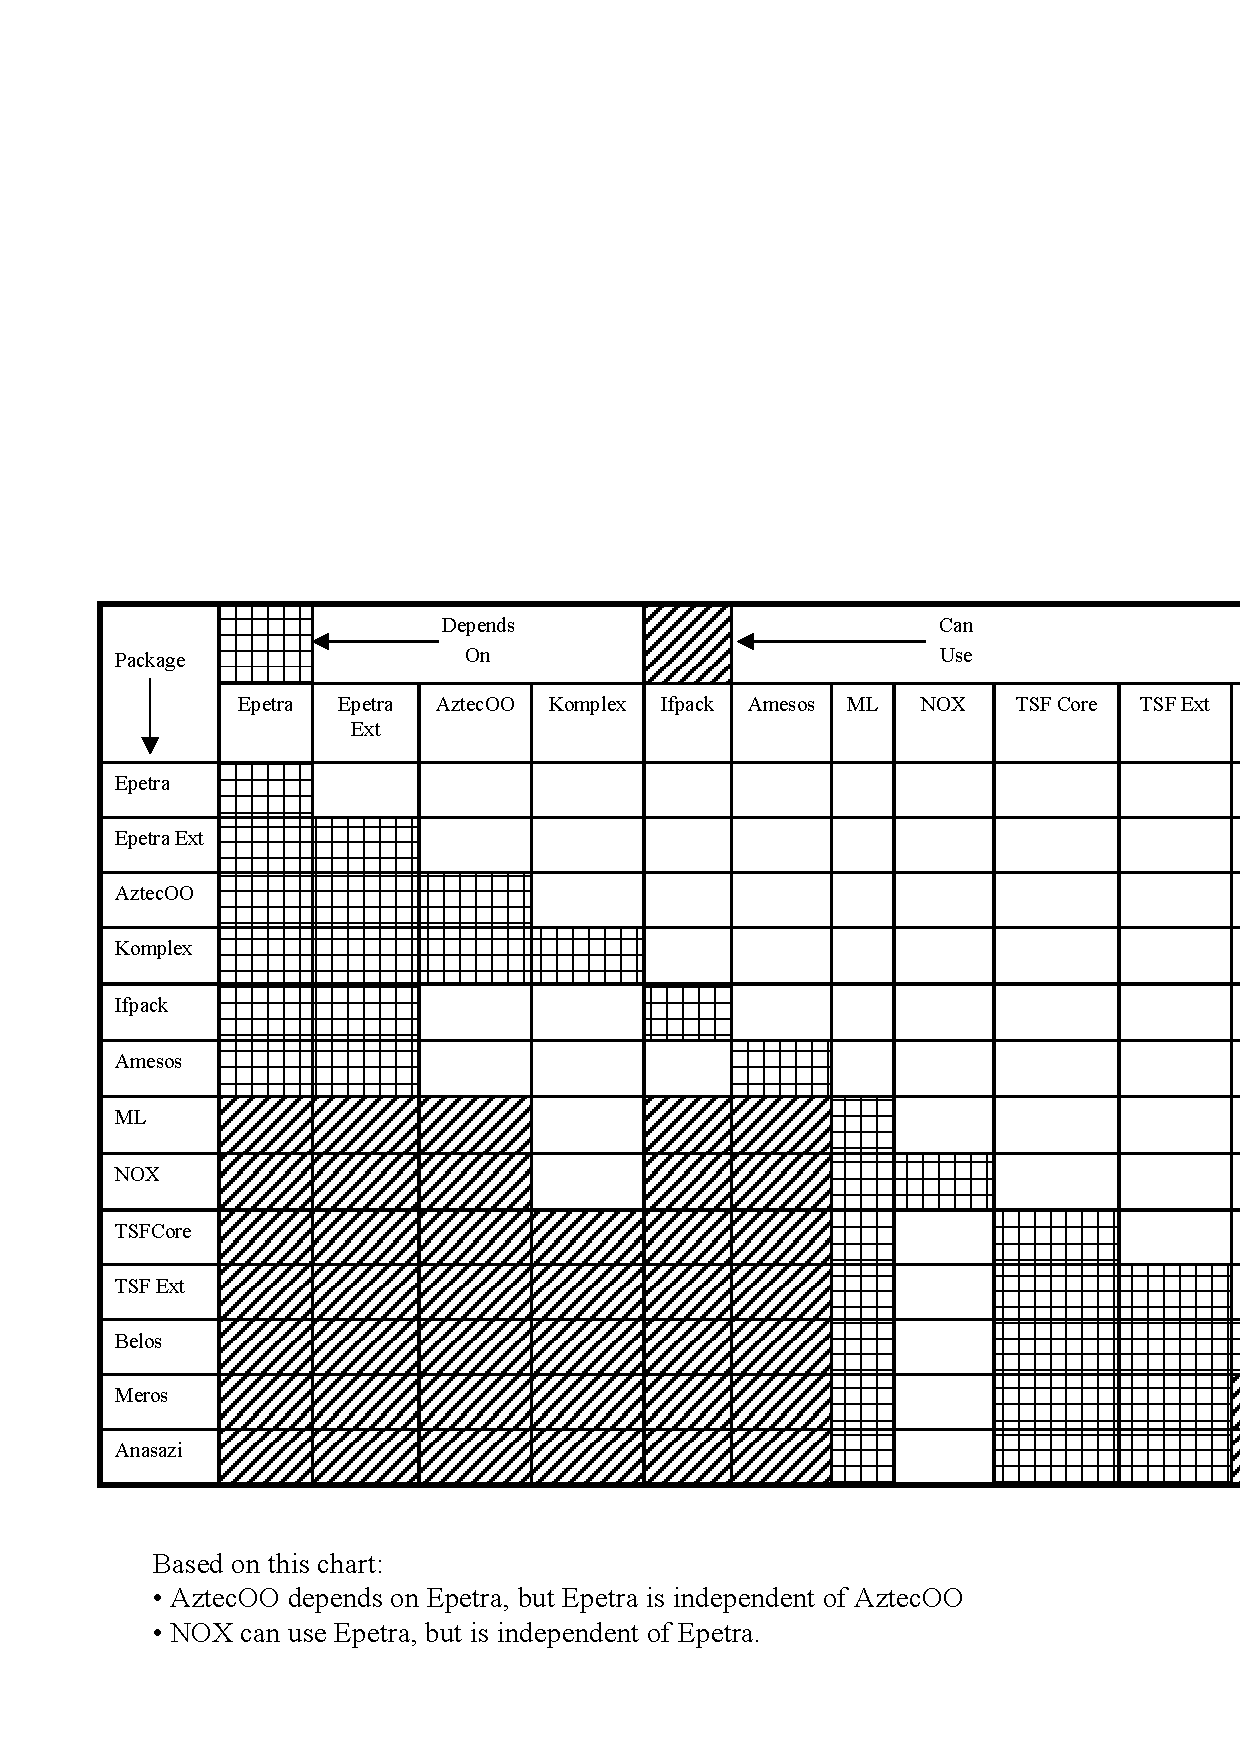
\includegraphics[height=6in,angle=270]{TrilinosPackageDependencies}
%\end{center}
\label{Figure:TrilinosPackageDependencies}
\caption{Current Trilinos Package Dependencies}
\end{figure}
collection of Trilinos packages depend on each other.

\section{Platform Portablility}
%	**(List platforms - encourage script submission)**

\clearpage
\bibliographystyle{plain}
\bibliography{TrilinosDevGuide}
\addcontentsline{toc}{section}{References}

\appendix
\section{Commonly Used CVS Commands}
\label{Section:CVS}
\section{Common Bugzilla Tasks}
\label{Section:Bugzilla}


\end{document}
